% THIS TEMPLATE IS A WORK IN PROGRESS

\documentclass[polish, a4paper]{article}
\usepackage[a4paper,left=3cm,right=3cm,top=3cm,bottom=1.5cm]{geometry}
\usepackage[T1]{fontenc}
\usepackage[polish]{babel}
\usepackage[utf8]{inputenc}
\usepackage{hyperref}
\usepackage{fancyhdr}
\usepackage{float}
\usepackage{graphicx}
\usepackage{titling}
\usepackage{wasysym}
\usepackage{caption}
\usepackage{pgfplots}
\usepackage{pgfplotstable}
\usepackage{filecontents}
\usepackage{csvsimple}
\usepackage{textcomp}
\usepackage{gensymb}
\usepackage{etoolbox}
%\usepackage{siunitx}
\graphicspath{ {./} }
\pagestyle{fancy}

\setlength{\droptitle}{-1in}

%\lhead{\includegraphics[width=0.2\textwidth]{nyush-logo.pdf}}

  \lhead{Maciej Kaszkowiak}
  \chead{Warstwa sieciowa}
  \rhead{
  151856}


%%%% PROJECT TITLE
\title{Warstwa sieciowa \\
        \Large \emph{Sprawozdanie nr 4 z przedmiotu Sieci Komputerowe}}

%%%% NAMES OF ALL THE STUDENTS INVOLVED (first-name last-name)
\author{Maciej Kaszkowiak, 151856, zadania wykonane 13 maja 2023}

\date{\vspace{-5ex}} %NO DATE


\begin{document}

\maketitle
%\thispagestyle{titlepage}

\tableofcontents

\newpage

\section{Zadanie 1}
\subsection{Zaloguj ruch przy pomocy programu wireshark. Jakie zazwyczaj są ustawione flagi w pakietach?}

Możemy zaobserwować 2 flagi w pakietach: "Don't fragment" oraz "More fragments".
\begin{figure}[H]
\centering
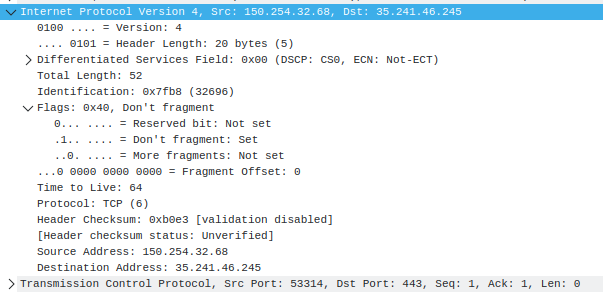
\includegraphics[width=\textwidth]{flagi.png}
\caption{Flagi w pakietach}
\end{figure}


\subsection{Powtórz ćwiczenie otwierając w międzyczasie jakąś stronę internetową przy użyciu protokołu https.}

Możemy zauważyć, że flaga Don't fragment w pakiecie została wyłączona.

\begin{figure}[H]
\centering
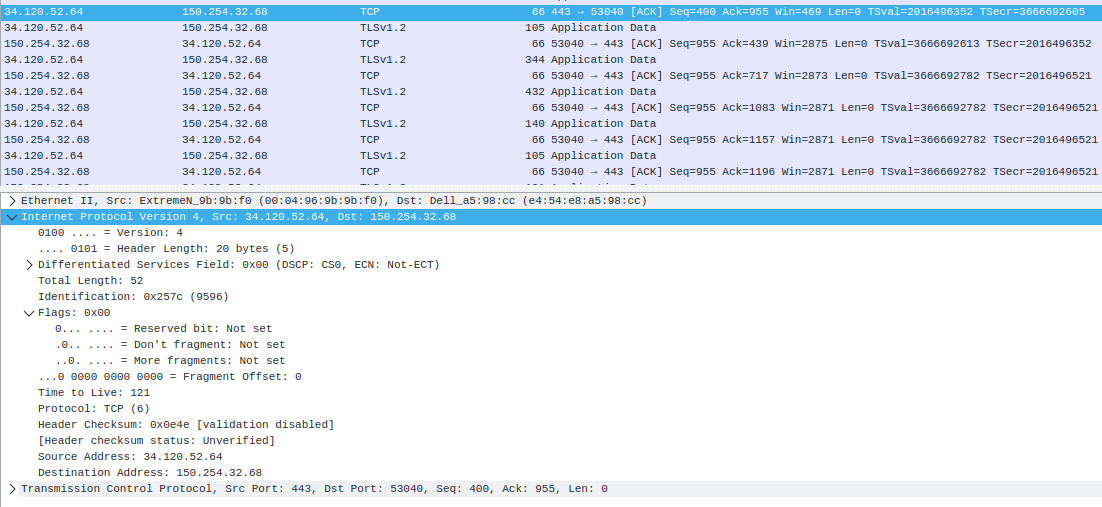
\includegraphics[width=\textwidth]{flagi 2.png}
\caption{Flagi pozwalające na fragmentację pakietu}
\end{figure}

\subsection{Powtórz ćwiczenie w międzyczasie wykonując polecenie ping -s 4000 na wybrany adres IP.}

Możemy zauważyć, że flaga Don't fragment w pakiecie jest wyłączona, a flaga More fragments w niektórych pakietach jest aktywna.

\begin{figure}[H]
\centering
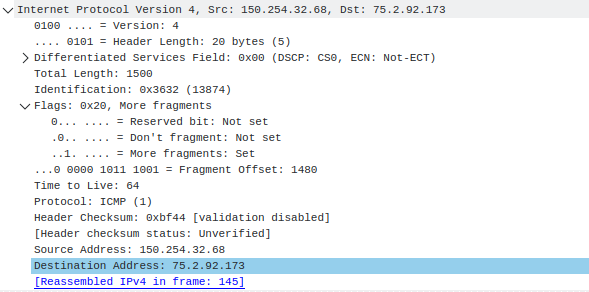
\includegraphics[width=\textwidth]{flagi 3.png}
\caption{Flagi w pofragmentowanym pakiecie}
\end{figure}

\section{Zadanie 2}
\subsection{Jak działa program traceroute (ewentualnie skorzystaj z opcji -I lub -T)?}

Program traceroute opiera się na mechaniźmie TTL w celu wyznaczenia poszczególnych węzłów na ścieżce pakietu wiodącego do wskazanego przez nas adresu IP. Program nasłuchuje na odpowiedzi ICMP informujące o porzuceniu pakietu ze względu na wyzerowanie jego wartości TTL. 

\begin{figure}[H]
\centering
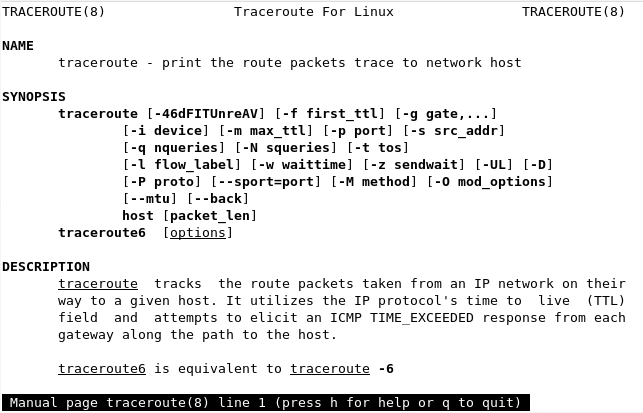
\includegraphics[width=\textwidth]{tracert.png}
\caption{Manpages programu traceroute}
\end{figure}

\subsection{Zaloguj ruch przy pomocy programu wireshark i zbadaj nagłówki pakietów generowanych przez program traceroute.}


\begin{figure}[H]
\begin{verbatim}
student@lab-sec-3:~> traceroute onet.pl
traceroute to onet.pl (99.83.207.202), 30 hops max, 60 byte packets
 1  150.254.32.65 (150.254.32.65)  1.528 ms  1.585 ms  1.681 ms
 2  150.254.30.129 (150.254.30.129)  1.044 ms  1.263 ms  1.501 ms
 3  * * *
\end{verbatim}
\caption{Wykonana komenda}
\end{figure}

Program generuje pakiety UDP z rosnącymi wartościami TTL, począwszy od TTL = 1. W odpowiedzi otrzymywane są pakiety ICMP informujące o porzuceniu pakietu.

\begin{figure}[H]
\centering
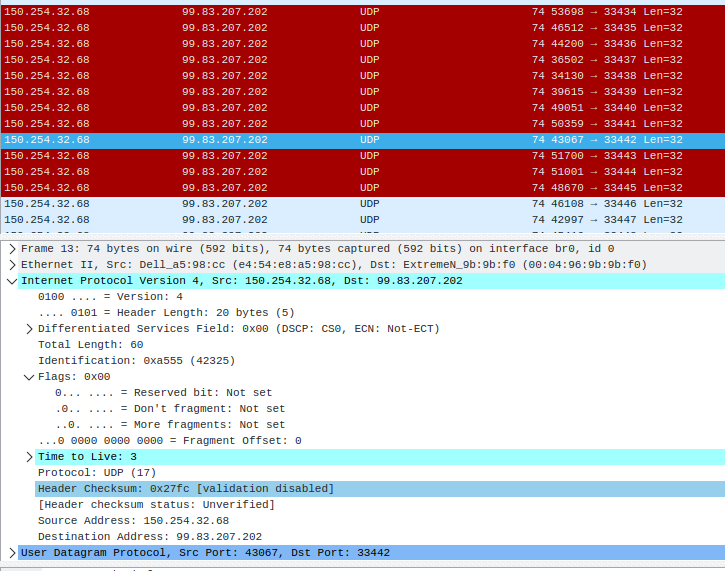
\includegraphics[width=\textwidth]{udp.png}
\caption{Nagłówki pakietów generowanych przez program traceroute}
\end{figure}


\section{Zadanie 3}
\subsection{Podłącz swój komputer (poprzez port p4p1) do koncentratora (na zapleczu).}

Podłączyłem swój komputer poprzez port o numerze 99 i interfejs p4p1. 

\subsection{Skonfiguruj interfejs p4p1, tak by wszystkie komputery w rzędzie działały w jednej sieci (unikalne sieci między rzędami).}

Połączenie działa:

\begin{figure}[H]
\begin{verbatim}
lab-sec-3:/homex/student # ip addr add 192.168.1.3/24 dev p4p1
lab-sec-3:/homex/student # ping 192.168.1.2
PING 192.168.1.2 (192.168.1.2) 56(84) bytes of data.
64 bytes from 192.168.1.2: icmp_seq=1 ttl=64 time=1.22 ms
64 bytes from 192.168.1.2: icmp_seq=2 ttl=64 time=0.634 ms
64 bytes from 192.168.1.2: icmp_seq=3 ttl=64 time=0.704 ms
64 bytes from 192.168.1.2: icmp_seq=4 ttl=64 time=0.496 ms
\end{verbatim}
\caption{Wykonana komenda}
\end{figure}

\subsection{Zbadaj jak zmienia się tablica ARP, gdy uruchamiasz program ping z argumentami będącymi adresami IP komputerów z Twojej sieci i adresami komputerów w innych rzędach (należących do innych sieci).}

Możemy zaobserwować, ze tablica ARP uzupełnia się po wykonaniu pingu do komputera w naszej sieci.

\begin{figure}[H]
\begin{verbatim}
lab-sec-3:/homex/student # arp -d 192.168.1.2
lab-sec-3:/homex/student # arp -n
Address                  HWtype  HWaddress           Flags Mask            Iface
150.254.32.65            ether   00:04:96:9b:9b:f0   C                     br0
150.254.32.120           ether   52:54:00:7d:97:53   C                     br0
192.168.1.1              ether   e4:54:e8:a5:98:c6   C                     br0
192.168.1.1                      (incomplete)                              p4p1
150.254.32.126           ether   00:25:64:3b:c1:d0   C                     br0
lab-sec-3:/homex/student # ping 192.168.1.2
PING 192.168.1.2 (192.168.1.2) 56(84) bytes of data.
64 bytes from 192.168.1.2: icmp_seq=1 ttl=64 time=1.44 ms
64 bytes from 192.168.1.2: icmp_seq=2 ttl=64 time=0.774 ms
^C
--- 192.168.1.2 ping statistics ---
2 packets transmitted, 2 received, 0% packet loss, time 1002ms
rtt min/avg/max/mdev = 0.774/1.104/1.435/0.330 ms
lab-sec-3:/homex/student # arp -n
Address                  HWtype  HWaddress           Flags Mask            Iface
150.254.32.65            ether   00:04:96:9b:9b:f0   C                     br0
192.168.1.2              ether   00:10:18:b4:e0:24   C                     p4p1
150.254.32.120           ether   52:54:00:7d:97:53   C                     br0
192.168.1.1              ether   e4:54:e8:a5:98:c6   C                     br0
192.168.1.1                      (incomplete)                              p4p1
150.254.32.126           ether   00:25:64:3b:c1:d0   C                     br0
\end{verbatim}
\caption{Wykonana komenda}
\end{figure}

Komputery w innych rzędach są nieosiągalne, przez co tablica ARP się nie uzupełnia - nie znamy adresów MAC nieosiągalnych węzłów.

\begin{figure}[H]
\begin{verbatim}
lab-sec-3:/homex/student # ping 192.168.5.14
PING 192.168.5.14 (192.168.5.14) 56(84) bytes of data.
From 150.254.4.66 icmp_seq=6 Destination Net Unreachable
^C
--- 192.168.5.14 ping statistics ---
9 packets transmitted, 0 received, +1 errors, 100% packet loss, time 8168ms

lab-sec-3:/homex/student # ping 192.168.5.15
PING 192.168.5.15 (192.168.5.15) 56(84) bytes of data.
From 150.254.4.66 icmp_seq=6 Destination Net Unreachable
From 150.254.4.66 icmp_seq=7 Destination Net Unreachable
^C
--- 192.168.5.15 ping statistics ---
7 packets transmitted, 0 received, +2 errors, 100% packet loss, time 6129ms

lab-sec-3:/homex/student # arp -n
Address                  HWtype  HWaddress           Flags Mask            Iface
150.254.32.65            ether   00:04:96:9b:9b:f0   C                     br0
192.168.1.2              ether   00:10:18:b4:e0:24   C                     p4p1
150.254.32.120           ether   52:54:00:7d:97:53   C                     br0
192.168.1.1              ether   e4:54:e8:a5:98:c6   C                     br0
192.168.1.1              ether   00:10:18:aa:bd:7c   C                     p4p1
150.254.32.126           ether   00:25:64:3b:c1:d0   C                     br0
\end{verbatim}
\caption{Wykonana komenda}
\end{figure}

Zadanie 4 nie zostało wykonane zgodnie z poleceniem prowadzącego.

\end{document}